% The blind-optimization curve as a native pgfplots graphic.
\begingroup
\tracinglostchars=0
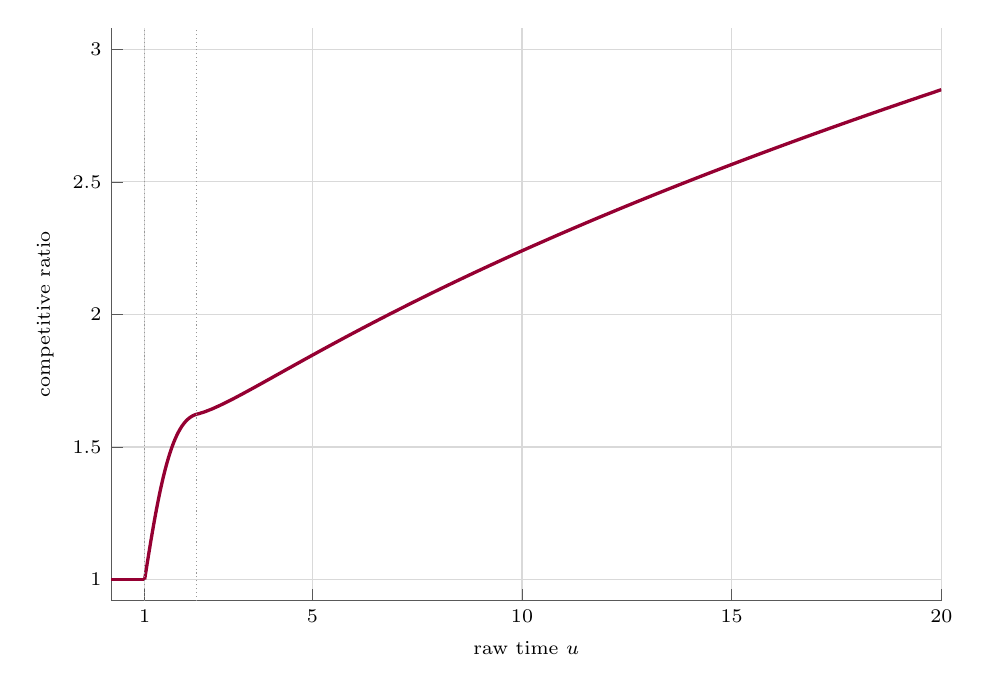
\begin{tikzpicture}
\begin{axis}[
  width=\linewidth,
  height=0.73\linewidth,
  xmin=0.2,
  xmax=20,
  ymin=0.92,
  ymax=3.08,
  xlabel={raw time $u$},
  ylabel={competitive ratio},
  xtick={1,5,10,15,20},
  ytick={1,1.5,2,2.5,3},
  tick label style={font=\scriptsize},
  label style={font=\scriptsize},
  grid=major,
  grid style={black!15},
  axis line style={black!65},
  tick style={black!65},
  axis x line*=bottom,
  axis y line*=left,
  samples=100,
  no markers,
]
% Blind optimization.
\addplot[purple!78!black,very thick,domain=0.2:1] {1};
\addplot[purple!78!black,very thick,domain=1:2.24697960372]
  {x^3/(x^2+(x-1)^3)};
\addplot[purple!78!black,very thick,domain=2.24697960372:20]
  {0.5*(1+sqrt((x^2+x-1)/(x-1)))};
\addplot[black!40,densely dotted,thin] coordinates {(1,0.92) (1,3.08)};
\addplot[black!40,densely dotted,thin]
  coordinates {(2.24697960372,0.92) (2.24697960372,3.08)};
\end{axis}
\end{tikzpicture}
\endgroup
